\chapter{Performance Evaluation}\label{ch:performance}

In this Chapter, we will evaluate the performance of the new CouchDB driver
comparing to the default disk implementation, that is currently used by Ganeti
for its storage requirements. Good benchmarks are non-trivial; each driver is
different, and different use cases need to tune different parameters. In next
sections, we will try to illustrate the benchmarking methodology of the diagrams
we are about to present, before we proceed to the detailed explanation of our
results.

The structure of this chapter is the following. Section~\ref{sec:specs} provides
details about the hardware and software on which we conducted our benchmarks,
while section~\ref{sec:bench} concentrates on the methodology behind our
measurements; the main factors we have taken into account in order to
decide which were the most interesting and applicable for Ganeti fields, were we
should evaluate our driver's performance. Finally, section
\ref{sec:perfom_couch} contains the actual performance evaluation of the CouchDB
driver. In each of its subsections concentrates on a specific field of interest
for the driver evaluation, which will subsequently lead us to the final
conjecture about how the driver responds to real-world workloads.

\section{Specifications}\label{sec:specs}

To evaluate our software tool, it was required to setup a Ganeti
cluster where our benchmarks would run. We decided to setup our testing cluster
into a virtualized environment. More specifically, we chosen \emph{Synnefo}
\flink{http://www.synnefo.org/}, an open source cloud software, to host our
testing environment. A bunch of reasons lead us to this decision. Firstly, as
Ganeti is a software tool for managing clusters of physical nodes, it is not a
facile task to obtain, setup, and maintain physical machines for the cluster
requirements. On contrast, using a virtualized environment makes it quite easy
to add and remove nodes from the cluster at will, without interacting with any
physical processes that would be running in a physical machine. It
provides a complete isolated environment where no one else can intervene with
our work. In addition, keeping up-to-date snapshots of our virtual nodes makes
disaster recovery quite a bit easier, and our cluster can be recovered in just a
few seconds in case of a hardware or a software failure. Moreover, it makes
incredibly simple and fast to modify the underlying hardware we use for our VMs,
through the hardware abstraction it is provided.

On the contrary, every virtualization solution comes with an additional overhead
in terms of computation, networking, and I/O operations. The overhead incurred
by virtualization has been the focus of many performance studies in the past,
including numerous of general-purpose benchmarks. A short review on those,
indicates an overhead below \emph{5\%} on computation~\cite{xen_art}, below
\emph{15\%} on networking~\cite{xen_art, diagnosing}, while the parallel I/O
performance losses  due to virtualization has been shown to be below
\emph{30\%}~\cite{xen_hpc}, respectively. Recently, there also has been occurred
a burst on the research activity related to the performance of using virtualized
resources in cloud computing environments~\cite{montage, Iosup_anearly,
parallel}, that provide additional metrics of the effects of using the cloud
computing services for running many types of scientific tasks.

In our case, the testing environment has been setup in a \emph{7-node}
cluster, where each node was armed with a \emph{24-core AMD Opteron(tm) 6172}
processor at \emph{2.10 GHz}, with \emph{189 GB} of primary memory, and
\emph{3.7 TB} of storage, running on a \emph{SMP Debian GNU/Linux} with
\emph{3.2.0-4} kernel in \emph{64-bit} mode. The virtualization software used,
was \emph{QEMU 1.7.0} with the aid of the \emph{KVM} kernel module. When used as
a virtualizer, QEMU achieves near native performance by executing the guest code
directly on the host CPU. The redundancy on the physical resources of the
nodes we setup our cluster, provides 1:1 mapping between the CPUs and vCPUS, as
for the primary memory too. This results to a
minimum performance overhead because there is no overcommitment in the physical
resources at all. On the contrary, we can not come through the overhead during
I/O operations with the disk and the network usage, but keeping in mind that both
of our drivers interact with the disk and make use of the network resources,
that overhead is linearly applied to each of them and will not affect the final
results. The specifications of each one of the VMs constituting our virtual
\emph{5-node} Ganeti cluster, where we conducted our benchmarks, are the
following.

\begin{table}[htbp]
  \centering
  \begin{tabular}{ | l | l | }
    \hline
    Component & Description \\ \hline \hline
    CPU & 8 x QEMU Virtual CPU Version 1.7.0 \\
    \hline
    RAΜ & 8192 MB  \\
    \hline
    Disk & 80 GB \\
    \hline
  \end{tabular}
  \caption{Test-VM hardware specs}
  \label{tab:hw-specs}
\end{table}

\begin{table}[htbp]
  \centering
  \begin{tabular}{ | l | l | }
    \hline
    Software & Version \\ \hline \hline
    OS & Debian 7.1 Wheezy Base System \\
    \hline
    Linux Kernel & 3.2.0-4-amd64  \\
    \hline
  \end{tabular}
  \caption{Test-VM software specs}
  \label{tab:soft-specs}
\end{table}

\section{Benchmark methodology}\label{sec:bench}

Real benchmarks require real-world load. We will try to test our driver on
real-world examples under situations when hundreds of clients try to interact
with the master daemon concurrently, meaning that the masterd has to deal with
them properly. Ganeti is a distributed software tool. So it is a premise to
scale well and perform-fast, when used in real production environments with tens
of nodes on each cluster.

There are a plenty of attributes affecting the performance of distributed
systems and multiple ``knobs" we could turn on to make a system perform better
in one area, but affecting another area when doing so. A use case is the CAP
theorem that was discussed in section~\ref{item:cap}. If we want our system to
scale out, for example, there are three distinct areas to deal with; increased
read and write requests, and data. In addition, reducing latency for a given
system, affects concurrency and throughput capabilities. These two examples are
graphically illustrated in Figure~\ref{fig:compr}.
Orthogonal to those attributes, there are many more factors that affect a system
such as Ganeti, and more of the figures below can be drawed, that display
different features such as reliability, simplicity, availability, and more.
CouchDB is very flexible and gives us enough tools to create a system shaped to
suit many, \underline{but not all}, of our problems.

\begin{figure}[htbp]
  \begin{center}
    \makebox[\textwidth]{%
    \subfloat[Performance: Throughput, latency, or concurrency]{{%
      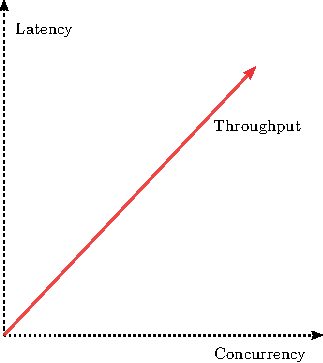
\includegraphics[width=0.35\paperwidth]{../figures/figure2.pdf}}}
    \qquad
    \subfloat[Scaling: read requests, write requests, or data]{{%
      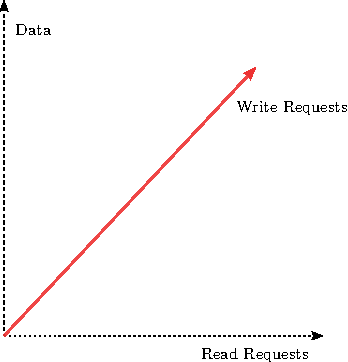
\includegraphics[width=0.35\paperwidth]{../figures/figure3.pdf}}}}
    \caption{Compromises of distributed systems\label{fig:compr}}
   \end{center}
\end{figure}

Keeping the above in mind, the benchmarks we have executed can be roughly
classified into four main categories, all of which having their own specific
goals.

The first category, aims to expose the effect in the job submission rate, when
the number of the master candidate nodes increases. In
order to effectively measure the overhead that is introduced with an increase in
the \texttt{candidate\_pool\_size} of the cluster, we will sent concurrently
\emph{errored} jobs to the master node, and then we will measure the rate that
Ganeti adds them to the queue. We intentionally chose to sent errored jobs,
because we simply want to observe how the job enqueue throughput of Ganeti
responds in various candidate pool sizes, and not any other factors that may be
affected by that type of measurement. The behavior we will observe, will also
indicate a suitable size of master candidate nodes, to conduct the rest of our
tests.

The second category, is a performance comparison test between the two driver
implementations; the default disk implementation that Ganeti currently uses, and
the CouchDB one. The comparison concentrates on the job submission rate, by
sending concurrently \emph{errored} jobs of various sizes similarly to the
previous category, but using a constant value of master candidate nodes instead,
the one that was determined previously. The aim is to measure the performance
against a tough workload, explain the differentiations, if any, that are
observed on both of the drivers, and expose the factors that have the greatest
impact on each of our drivers.

The third category deals solely with the configuration data management. We
measure the performance of the configuration related write requests, on several
file sizes, and in clusters with various candidate pool sizes, to examine the
bottlenecks on having a single configuration file on big production clusters
mainly. We will investigate all the factors that are delaying the update of the
configuration file, on both of the drivers, and then we conduct a comparison
test among them.

Lastly, in the forth benchmark category, we position the CouchDB and the disk
driver in a real-world scenario; an attempt to create a bunch of instances and
compare the total execution time of those jobs on each implementation. We aim to
present the overall performance of each driver, and explain any differentiations
that may arise.

\section{Evaluating CouchDB}\label{sec:perfom_couch}

The overview of the benchmark methodology we provided, points out the various
situations along with different metrics and workloads where we tested our
implementations, in order to measure accurately their performance. The
abovementioned categories, are presented in more details in the upcoming
sections.

\subsection{Impact of the candidate pool size}\label{subsec:cand_size}

This category is a sort of an introductory section for the rest of our tests.
Ganeti maintains a set of master candidate nodes, those that also contain a copy
of the full cluster configuration, i.e., configuration and jobs files. The
existence of those nodes has a great impact in the overall performance of the
cluster, due to the fact that each modification in a disk configuration file
causes a copy of it file to the candidate nodes. Creating a cluster with no
master candidates at all is a risky attempt, because in case of a master
failure all the cluster information will be lost. On contrast, maintaining a lot
of master candidate nodes is a redundant waste of resources, as modifications
have to be replicated to more nodes. We would ideally want to find out the set
of master candidate nodes that fits a production environment, in terms of having
the less impact in the cluster performance, and reducing the probability of a
cluster failure.

In order to decide which is the most appropriate candidate pool size, we
proceed with the following scenario. We sent jobs concurrently to Ganeti with
varying candidate node numbers, and we measure the rate in which jobs are
submitted to the queue, for each case.
This metric is the job enqueue throughput, and denotes the average number
of jobs that are added to the queue per second. It is a representative metric
for our purpose, because every new entry to the job queue will also be
replicated to the master candidate nodes before the operation is declared as
successful. Since we are just
interested for the enqueue rate, we decided to submit jobs that will
never be executed and will be declared as \emph{errored}. An example of those
jobs is the modification of an instance that does not exist in the cluster. The
jobs will be normally inserted to the queue and replicated to the candidate
nodes, but when they will start their execution, they will immediately fail as
\emph{errored}.

Jobs have been sent to Ganeti in batches of \texttt{10}, \texttt{20},
\texttt{30}, \texttt{40}, \texttt{50}, \texttt{100}, \texttt{150}, and
\texttt{200} jobs. We ran that benchmark in a \emph{5-node} cluster consisting
of \texttt{none},
\texttt{one}, \texttt{two}, and \texttt{four} master candidate nodes, and the
whole procedure has been repeated ten times in total. Since Ganeti writes every
information to filesystem and then distributes it to the candidate nodes, there
is a lot of disk and network I/O interaction. As a result, we expect a short of
deviation in our sample data values because there are external factors that may
affect the performance. The ``outliers" values that may arise should also be
included in the final results, because are part of the Ganeti behavior.
Consequently, we believe that the \emph{mean} value of our distribution is the
most appropriate metric for our case, because is a metric that represents the
\emph{central tendency} of the distribution by taking into account the whole
data information.

The benchmark outputs are summarized in two figures. Figure~\ref{fig:mc_comp},
presents the total results in a normal \emph{line-points} plot style, while
Figure~\ref{fig:const_jobs} concentrates on the heavier workload of our
benchmark that are closer to a real-world environment, in a clustered
\emph{bar-graph} plot.

\begin{figure}[htbp]
  \begin{center}
    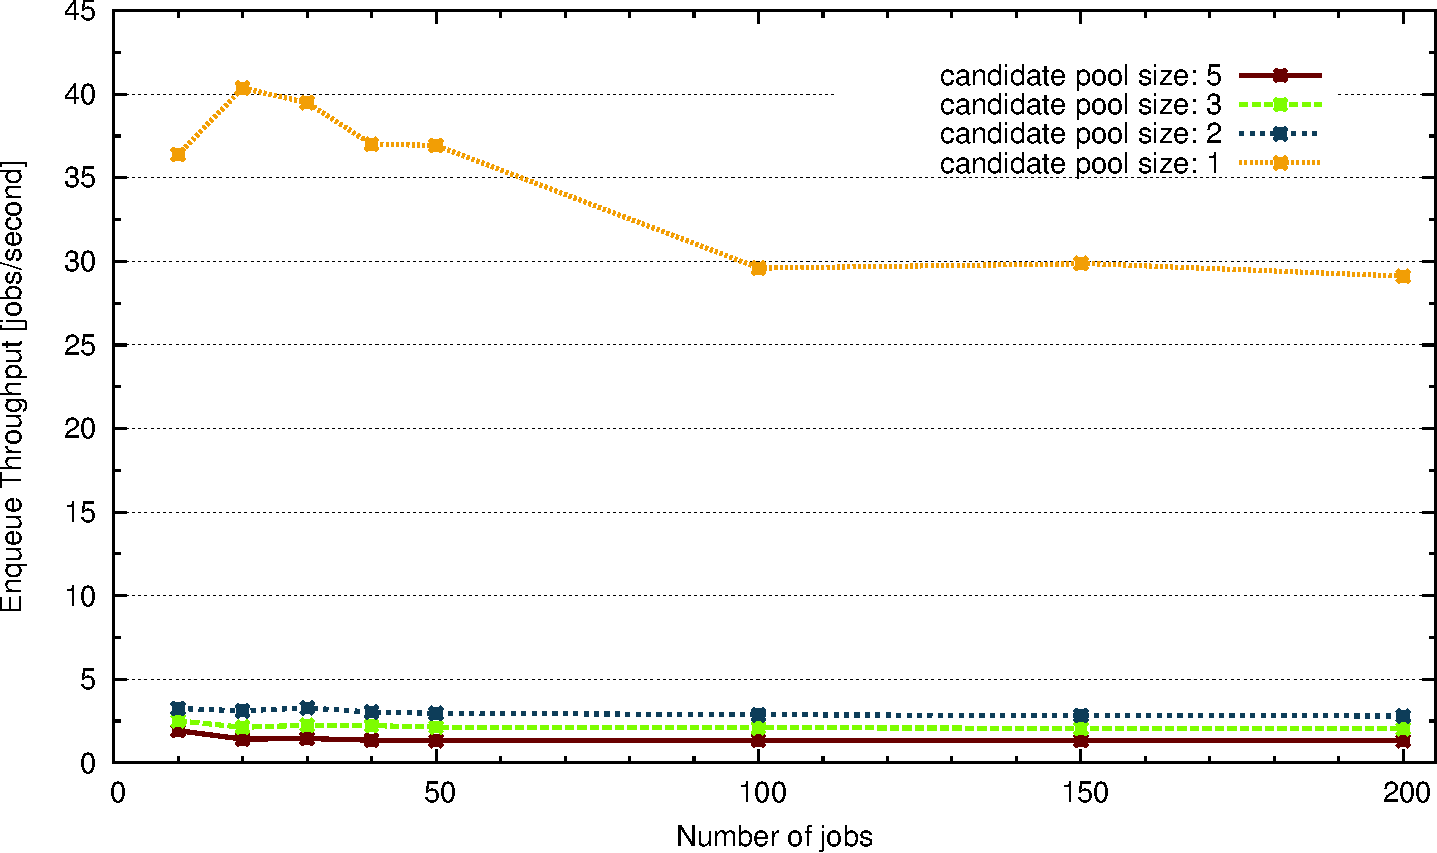
\includegraphics[width=1.0\maxwidth]{../figures/mc_comp.pdf}
    \caption{Job submission rate per number of candidates}
    \label{fig:mc_comp}
  \end{center}
\end{figure}

\begin{figure}[htbp]
  \begin{center}
    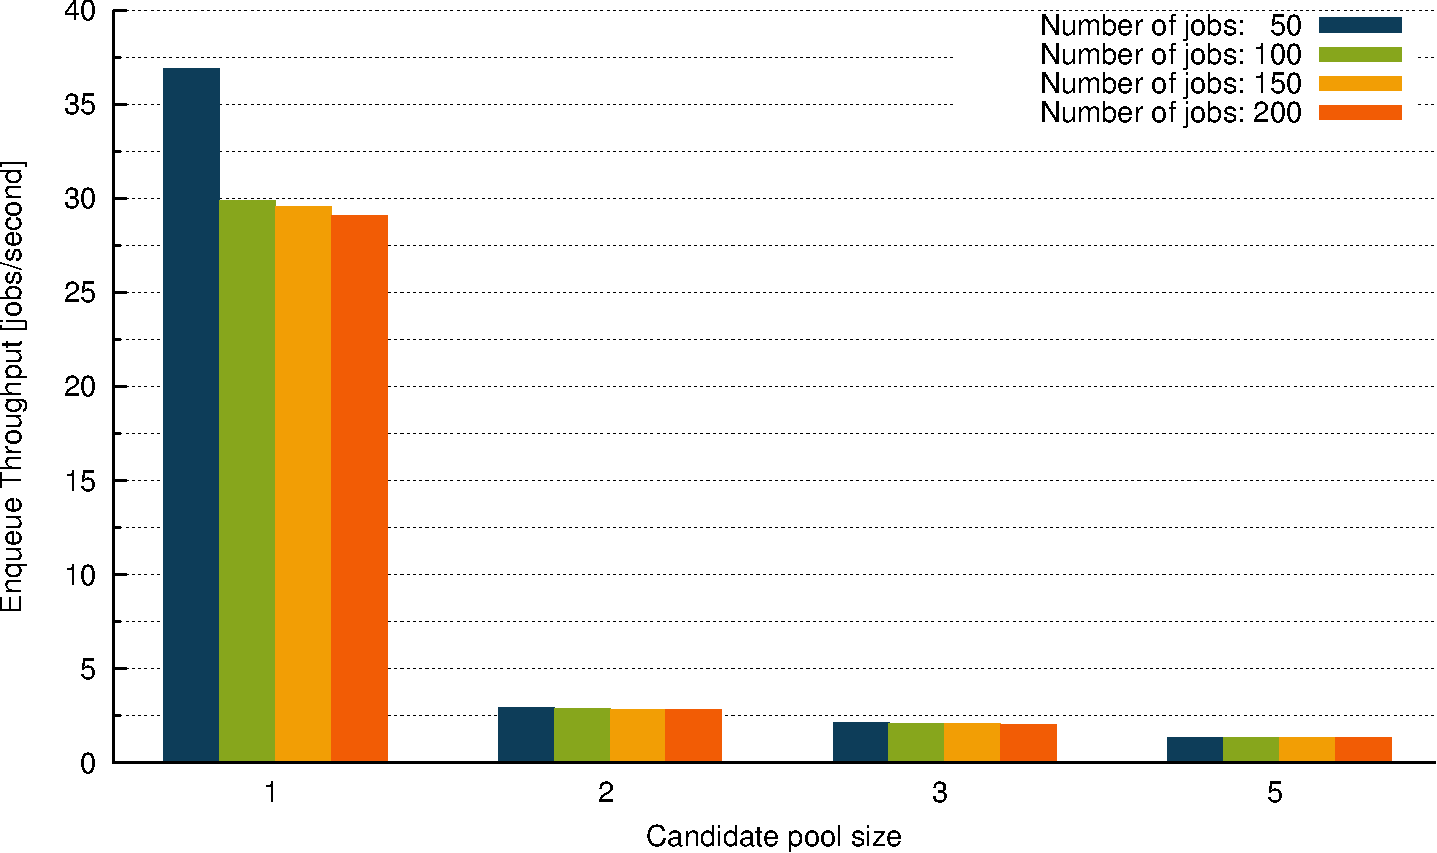
\includegraphics[width=1.0\maxwidth]{../figures/const_jobs.pdf}
    \caption{Job submission rate per number of candidates \#2}
    \label{fig:const_jobs}
  \end{center}
\end{figure}

\textbf{Performance Analysis}

There are several interesting points that we can conclude from these diagrams,
which we will address below. The most obvious observation is the significant
drop in the throughput performance, as we increase the master candidate
nodes of the cluster. Furthermore, in case of no master candidate nodes, the
distribution appears skewed characteristics and visible differentiations in the
throughput performance, something that is not observed when the candidate pool
size is increased. A closer explanation of those points follows.

In both figures, there is an obvious relationship between the job submission
rate and the number of master candidates that Ganeti maintains. As we stated in
the Caveats section, i.e., \ref{sec:caveats}, Ganeti writes jobs to disk and
then concurrently replicates them to the master candidates. The performance
slowdown of the replication process is displayed in these figures. With a single
master candidate node, we have a drop in the throughput of about \emph{8 times}
comparing to the case of no master candidates. An additional increase in the
candidate number, has no significant performance drop. This is an expected
behavior because Ganeti uses a multi-node RPC call to update the files in the
candidate nodes. This small dropdown is totally expected due to the checks that
Ganeti does after each RPC call, to get informed about the success, or not, of
the operation.

Another interesting finding from our results, are the ``outliers" that were
observed in the output sample data. When we ran the benchmarks in a cluster with
no master candidates, the data tended to have a more sparse behavior than in a
cluster with one, or more, candidate nodes. In order to make that variation
visible to the reader, we calculated the \emph{standard deviation} metric of our
distribution, which shows how much dispersion from the average value exists, and
we present it in Figure~\ref{fig:std} to justify our claim. The question that
may arise is: \emph{Why the deviation exists only in the case of a cluster with
no candidates}. The submission rate of Ganeti is the rate that the data are
written to disk, and replicated to the candidate nodes. Obviously, the disk and
network I/O are some of the factors that affect our results. As we know, Ganeti
writes the jobs to its queue, so when a worker thread grubs a job for execution,
it will subsequently update the job file in disk too. This causes
a lot of congestion in the job queue lock both from the master thread and the
job queue workers. The order that the workers grub jobs for execution causes
those differentiations in the throughput performance, in case of
no master candidates. On contrast, when the cluster contains master candidate
nodes, we have a totally smooth distribution with data around the mean value.
This behavior is justified by the replication process of the job files to the
candidate nodes. It is a quite time-consuming operation, that covers the
rest operations that are executed, and actually determines the result's form. At
this point, many types of measurements can be taken that will clarify those
claims and probably will expose more, but are out of the scope of this document
and this test category specifically, and we will not expand further.

\begin{figure}[htbp]
  \begin{center}
    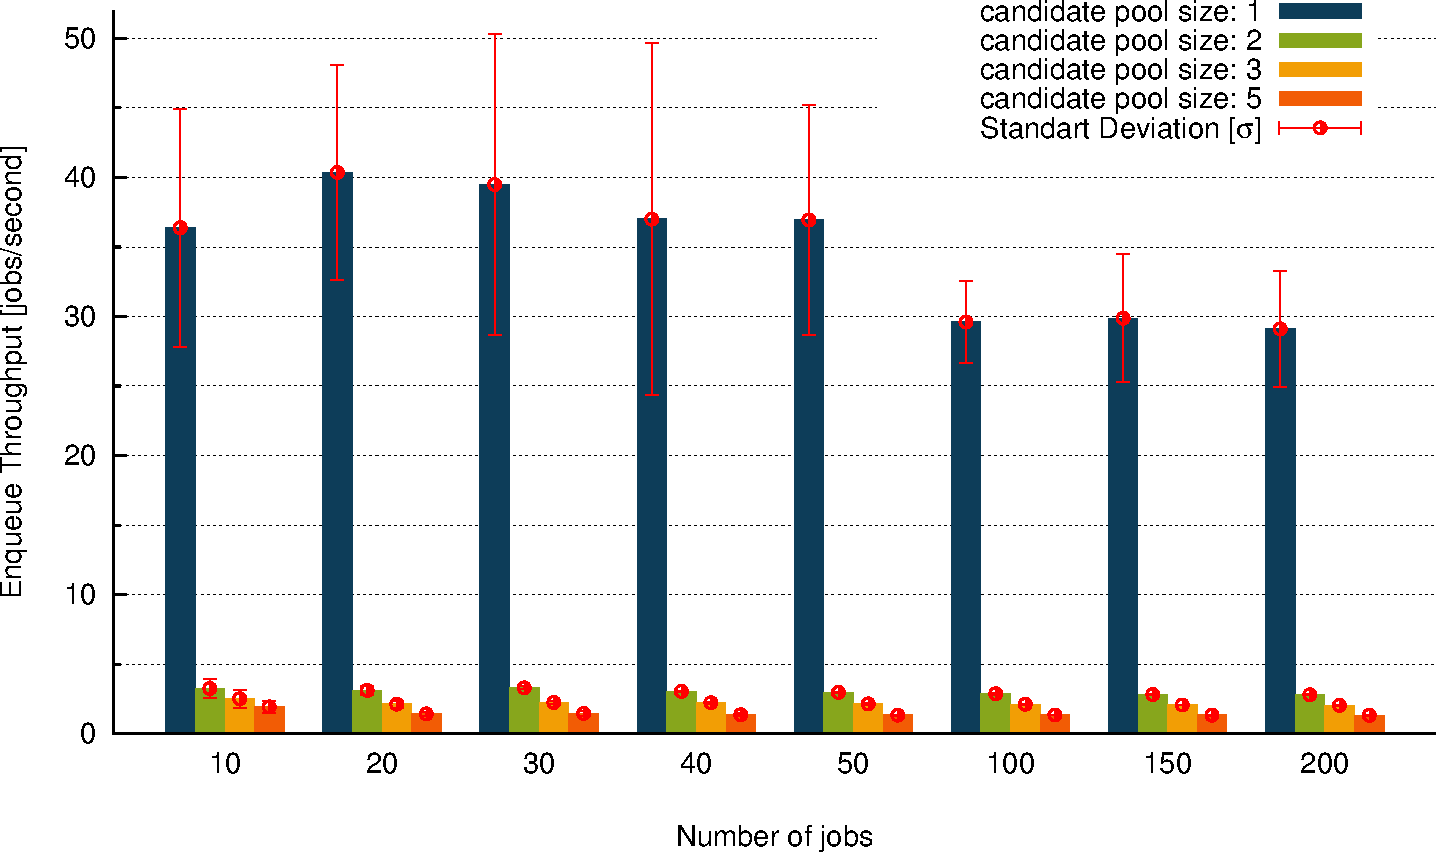
\includegraphics[width=1.0\maxwidth]{../figures/std.pdf}
    \caption{Standard Deviation [σ] of the job submission rate}
    \label{fig:std}
  \end{center}
\end{figure}

Summing up, from the results we presented, we believe that having a cluster with
two candidate nodes is the best choice to conduct the rest of our benchmarks. It
is also a choice that reflects a real production environment because it provides
the appropriate backup degree in case of a hardware failure, and also does not
have great performance impact comparing to a cluster with a single candidate
node.

\subsection{Comparison of the job submission rate}\label{subsec:enqueue_rate}

To some extend, we already discussed about the job submission performance rate
of Ganeti's default disk storage implementation, and we explained some of the
drawbacks that start to appear as the candidate pool size increases. In this
category, we make use of exactly the same metrics that we used in the previous
one, with the difference that the tests are conducted in a cluster with a
candidate pool size equal to \emph{three} nodes, as we determined in the first
benchmark category.

It is the first category where we actually compare the two driver
implementations, and we explain the main factors that affect their performance.
The results are summed up in two figures. Figure~\ref{fig:comp}, contains the
comparison of the job submission rate between CouchDB and the disk storage type,
while Figure~\ref{fig:couch_comp} presents the comparison of the CouchDB driver
performing under different socket options.

\begin{figure}[htbp]
  \begin{center}
    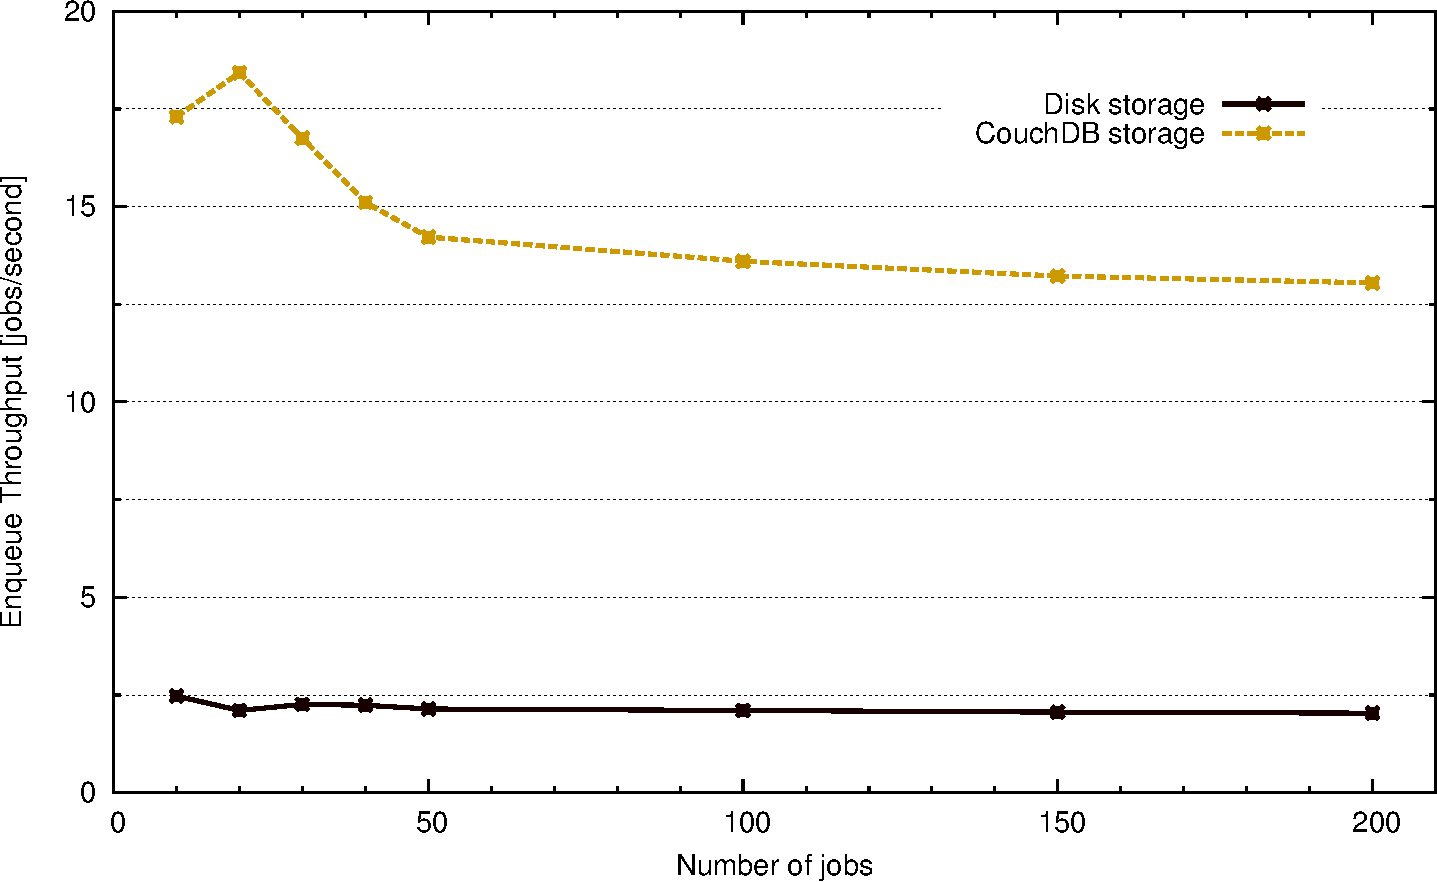
\includegraphics[width=1.0\maxwidth]{../figures/comp.pdf}
    \caption{Comparison of the throughput performance}
    \label{fig:comp}
  \end{center}
\end{figure}

\begin{figure}[htbp]
  \begin{center}
    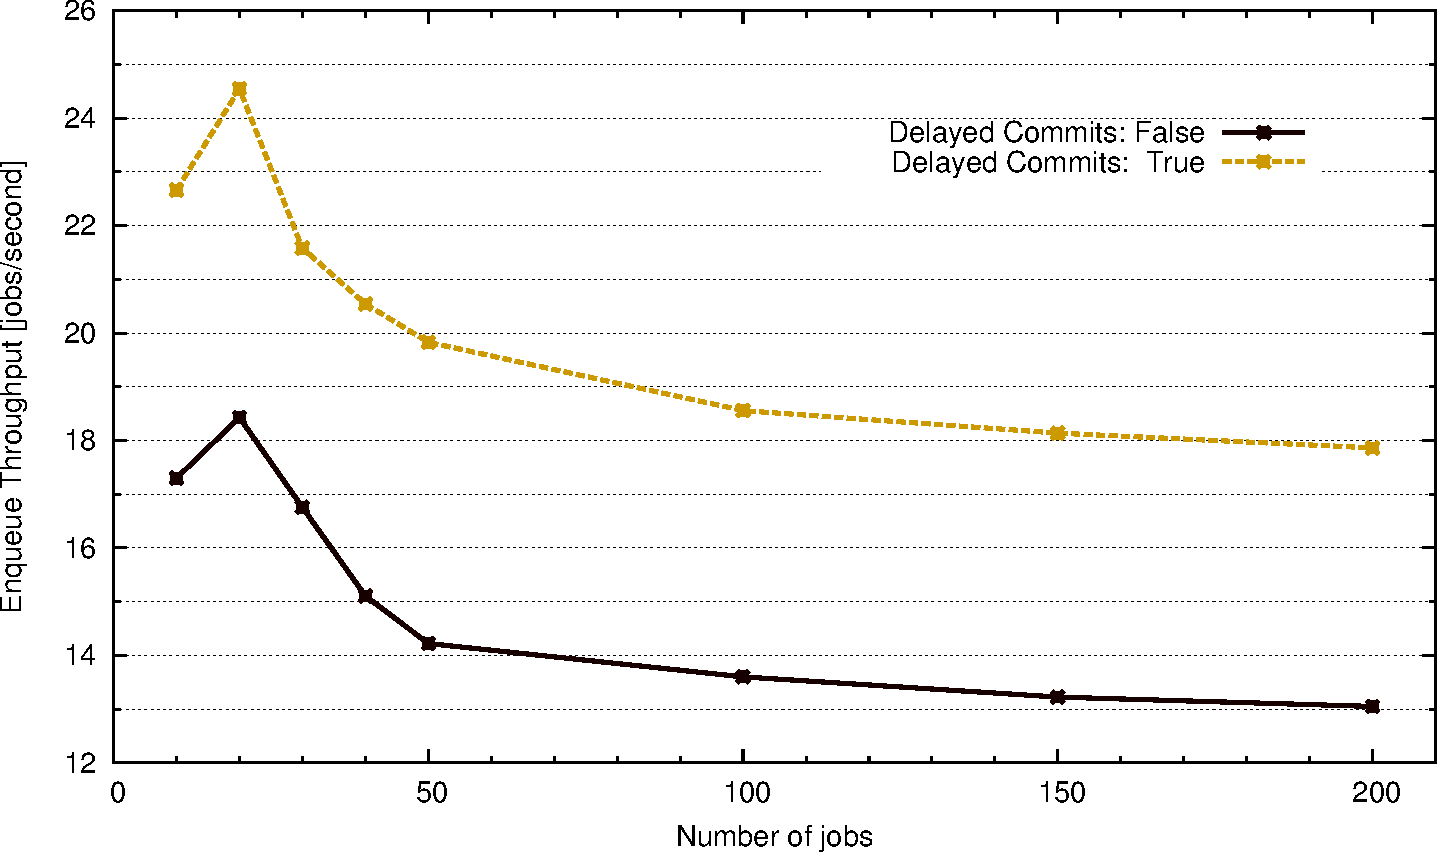
\includegraphics[width=1.0\maxwidth]{../figures/couch_comp.pdf}
    \caption{Throughput performance of CouchDB on various socket options}
    \label{fig:couch_comp}
  \end{center}
\end{figure}

\textbf{Performance Analysis}

Before we proceed with the interpretation of the diagram results, we have to
mention that the metrics we used, are exactly the same as in the first benchmark
category, and the final values correspond to the \emph{mean} value of every
distribution too.

Figure~\ref{fig:comp}, is the first performance comparison test that we
made between the two peers. The initial results look very promising. In a
\emph{5-node} cluster with two master candidate nodes, we have a speedup in the
job submission rate at about \emph{7-times} in the CouchDB driver, comparing to
the default disk storage implementation. The job submission rate has impact in
the overall job execution duration, as we will show in the last benchmark
category, and also reduces the timeouts happen in the LUXI server when many
clients try to submit jobs to Ganeti. We extensively talked about the reasons
that performance drops in a Ganeti cluster when jobs are saved to disk, in the
first test category. Now we are going to have a closer inspection in the
factors that prevent CouchDB from presenting similar behavior.

We discussed a lot about how Ganeti distributes the configuration files
to the candidate nodes, and we presented the performance impact of this
operation in the first category's figures. One of the main reasons we have
chosen CouchDB for Ganeti, is the replication feature, as it was discussed in
section~\ref{item:replication}. CouchDB is a database the replicates, and with
this term we mean that its fundamental function is to provide a simple, fast,
and convenient way to \emph{synchronize} two or more CouchDB databases.
Replication is handled completely by a separate process, external to Ganeti,
which listens on changes to the \emph{source} database, and replicates them to
the \emph{targets}. Obviously, the source refers to the master database, while
the targets are the databases of the candidate nodes. The \texttt{replicator}
process listens continually to the source's \texttt{\_changes} feed, and a new
modification to the source will immediately be replicated to the candidate
nodes. In order to ensure safety, CouchDB makes an \emph{fsync} call before a
\emph{201 Created} request is returned to the client. As soon as the
nodes are ``up" and running CouchDB will replicate, and there is no need to make
extra checks similar to the RPC checks that Ganeti has to make to find out that
the updates have reached a majority of the nodes, before declaring the
operation as successful. Instead, it is sufficient to check that the CouchDB
servers in the candidate nodes are accessible. This operation can be handled by
individual clients, independent to Ganeti that will not affect the performance,
and is an issue that is expected to be fixed in a future driver version, as we
will discuss in the Conclusion, i.e., Chapter~\ref{ch:conclusion}.

Besides the comparison test between the two implementations, we also make
a comparison test for the CouchDB drive,r on various socket options that CouchDB
provides, and have a great impact in the overall performance of the tool.
Figure~\ref{fig:couch_comp} shows this performance comparison test, on the
\texttt{delayed\_commits} attribute of CouchDB. When we set this attribute to
\texttt{True}, it is observed a further increase in the throughput performance
at about \emph{9-times} comparing to the default disk implementation, and at
about \emph{35\%} comparing to the CouchDB driver with this attribute set to
\texttt{False}. Delayed commits is probably the most important CouchDB
configuration setting for performance. When is set to true (the default),
CouchDB allows operations to be run against the disk without an explicit
\emph{fsync} call after each operation. Fsync operations take time in order to
complete, and calling them on each update limits the CouchDB performance for
sequential writers. It is clear that setting this option to true, opens a
window for data loss, because data are being kept in a write buffer and are
fsync-ed after a certain amount of time, or when the buffer is full. Ganeti is
an environment where we absolutely need to know when the updates have been
received, so we set this attribute to false, by default. The aim of this
test, is to expose an important setting of CouchDB that could be enabled
periodically, in several cases, like in a situation with an overloaded master
daemon, and then disabled at will. It is up to the cluster administrator to
measure the tradeoff between loosing some data in case of a hardware failure,
and the ``relief" that the performance improvement will bring to the cluster.

To achieve the results we presented for the CouchDB driver, another
important configuration option must be modified, related to the TCP buffering
behavior. This is the \emph{nodelay} option which must be set to \texttt{True},
in order to disable the \emph{Nagle's algorithm}~\flink{http://en.wikipedia.org/
wiki/Nagle\%27s\_algorithm}, which introduces an additional delay when using
keep-alive HTTP-connections. By setting this option to true, the
\emph{TCP\_NODELAY} option is turned on for socket, which means that even small
amounts of data sent to the TCP socket, like the reply to a document write
request, or reading a very small document, will be sent immediately to the
network. They will not be buffered hoping that it will be asked to send more
data through the same socket in order to transfer them all at once. The main
reason that this important option is disabled by default, is that the last
releases of CouchDB ships with a more recent version of the HTTP server library
\emph{MochiWeb}~\flink{https://github.com/mochi/mochiweb}, which by default sets
the \emph{TCP\_NODELAY} socket option to false.

\subsection{Comparison of the config.data performance}\label{subsec:config_perf}

The CouchDB driver, besides the alternative storage solution that provides to
the configuration files of Ganeti, also introduces a variation in the
way it handles the \texttt{config.data} file, as it was extensively discussed
in Section~\ref{sec:config}. The ultimate aim of this category is to compare the
performance of the two alternative implementations of handling the configuration
file, but before we reach to this point, we will investigate in deep all the
factors that affect the configuration file performance, and that were discussed
in Section~\ref{sec:caveats}.

In this category we will present three diagrams in total. The first two
of them [\ref{fig:total-cfg}, \ref{fig:couchdb}], one for each driver,
show the total execution duration of the \texttt{\_WriteConfig} method, and all
the sub-method calls that are been made. This is the responsible method for
applying the changes of the configuration file to the permanent storage, and
replicate them to the master candidate nodes.
Every operation that modifies the cluster state calls this function to
make the changes permanent. It is the most time consuming function related to
the configuration file, and has a great importance in the performance of Ganeti,
because is must be called with the \texttt{ConfigWriter} lock held in exclusive
mode, which starts to become a bottleneck when a huge number of jobs is in
execution. If we manage to reduce the time the lock is held by the workers, we
will also reduce some of the congestion in the config lock. The last diagram
[\ref{fig:comp-cfg}], is the actual performance comparison plot between the two
implementations.

The benchmarks of this section have been conducted on a cluster with a candidate
pool size equal to \texttt{one}, \texttt{three}, and \texttt{five} nodes,
respectively. In order to measure the performance of the \texttt{\_WriteConfig}
method, we intentionally increased the size of the \texttt{config.data} file,
from \texttt{100 KB} up to \texttt{5 MB}. A cluster with about \emph{2.000}
instances has a configuration file of around \texttt{5 MB}, which corresponds to
a real workload for a production environment. Our test concentrates on modifying
a parameter of a single configuration object. We chose an instance object as a
use case. Starting, restarting, or stopping an instance is a quite commonly used
operation, that while it aims to modify a single field of the instance object,
the whole configuration object is flushed to disk, and moreover the
\texttt{ssconf\_*} files are not affected; a variance that we do not want
to take into account in this test category. The test was repeated \emph{20}
times for each pair, and we find it appropriate to make use of the
\emph{trimmed mean} value of our distribution. The trimmed mean is a method of
averaging, that removes a small percentage of the largest and the smallest
values before calculating the mean. This method aims to reduce the effects of
the outliers on the calculated average, and stated as mean trimmed by
\emph{X\%}, where \emph{X} is the sum of the percentage of observations
removed from both the upper and lower bounds. In our case, we trimmed the mean
by \emph{20\%}. The reason we did not calculate the normal mean value, is that
we wanted to reduce the effects of the outliers that were observed, and to
obtain a more accurate average performance overview, for both the
implementations.

\bigskip
\textbf{Performance Analysis}

In the begging of our analysis, we will take a closer inspection on all the
factors related to the performance of the write operation of the
configuration file. An operation that affects the configuration state, passes
from the following execution phases in general. Firstly, some preliminary checks
are being made on the object that it is requested to change, and then the
update of the in-memory representation of the \texttt{config.data} object
follows. Then the \texttt{\_WriteConfig} method is called, which flushes the
updates to disk, and replicates them to the candidate nodes. This method
consists of a number
of time-consuming sub-method calls that affect the overall performance of any
cluster operation that modifies the configuration file. These calls contain the
verification of the config object for configuration errors, to maintain the
consistency of the object, and is named \texttt{\_UnlockedVerifyConfig}, the
serialization of the config object in order to be prepared for applying the
changes to disk, through the \texttt{serializer.Dump} call, and then the actual
flushing of the in-memory object to disk, using the \texttt{utils.SafeWriteFile}
function call. Finally, the modifications have to be replicated to the candidate
nodes with the \texttt{\_DistributeConfig} method. All these operations are
affected from the size of the configuration file, and from the candidate pool
size as well. Figure~\ref{fig:total-cfg}, extensively examines this behavior.

From Figure~\ref{fig:total-cfg}, the following conclusions can be made. The most
time-consuming method, is the serialization of the configuration file. It
is a totally independent cost from the candidate pool size, but it is 100\%
bounded with the size of the file. The file is stored in
memory as a \texttt{ConfigData} object, a generic config object defined by
Ganeti. In order to be saved to disk, it must be transformed to a string format,
and this is the role of this method. The cost of the file replication to the
candidate nodes is increases along with the number of master candidates, and the
size of the file too. In the same sense, the verification check consumes a lot
of time in bigger file sizes because it traverses the whole file, same as the
time of the function that applies the changes to disk, but with the difference
that even in bigger file sizes it
does not consume a noticeable amount of time. From this diagram it is understood
that in a cluster with three candidate nodes, even from a file of \emph{1.0 MB}
in size, it takes at about \emph{1 sec} to complete a single operation.
If we combine it with the congestion on the config lock, we can see
the great impact of that delay in the overall cluster's performance.

It is obvious that a single configuration file comes with a number of
disadvantages. Modifying a single field of the file requires the serialization
of the whole config object and the distribution to the candidates, as well. This
approach reduces the cluster performance due to the increased operational cost
that is implied. In Figure~\ref{fig:couchdb}, we will present a different
approach that the CouchDB driver introduces, by conducting the same test on the
\texttt{\_WriteConfig} method of the CouchDB driver.

In Figure~\ref{fig:couchdb}, we observe a great improvement in the total
execution duration of updating the configuration file. This differentiation can
be justified by the different approach of CouchDB of handling the config object.
The configuration file has been separated to its sub-components, as
we extensively discussed in section~\ref{item:config}. Modifying an instance, a
node, and generally a single object of the configuration file, does not updates
the whole object to disk, but only the single object we want to.
Moreover, the serialization cost does not
implies anymore. The transformation of an object before it is written to disk
is a simple conversion to dictionary, and it is part of the
\texttt{utils.WriteDocument} method. Since we convert only few kilobytes each
time the cost is negligible. The distribution cost is also disappears due to
the different approach of CouchDB on handling the replication process, as we
already extensively explained. The verification cost is the only one that does
not changes, since we continue to verify the whole in-memory configuration
object.

The last diagram we are going to present in this category, is presented in
Figure~\ref{fig:comp-cfg}. It displays the total execution duration of an
instance modify operation. It is a representative job, as all Ganeti operations
modify a specific field of the configuration file. The same output would appear
if we were modifying a node, a network, or a nodegroup. As we said in the
\emph{Implementation Details} section of the CouchDB driver, i.e., Section
\ref{sec:couch_details}, every update causes two consecutive object updates to
the CouchDB server. One for the cluster general information, and one for the
object we want to change. In this figure, we present the total execution time
for CouchDB, that is the aggregated execution duration of the two objects.
Even with this overhead the difference of flushing the whole file to disk
comparing to the single object that is updated is significant. For example, for
a file of \emph{2 MB} in size, we have at about \emph{5-times} increase in the
performance of CouchDB, while the gap is widening as the file size further
increases.

\begin{figure}[htbp]
  \begin{center}
    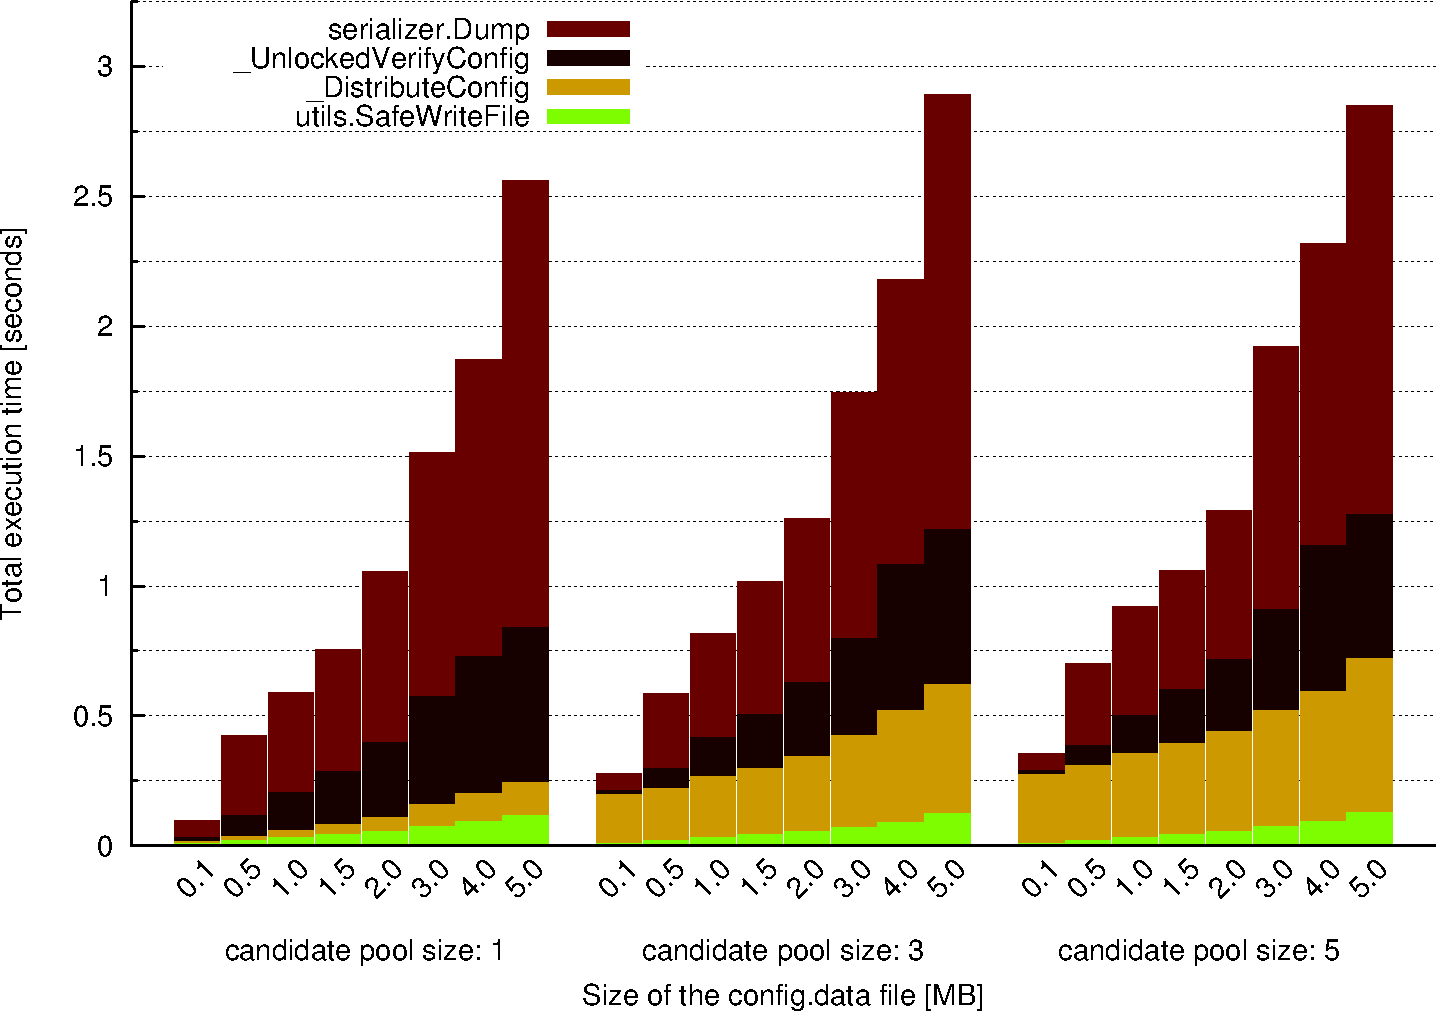
\includegraphics[width=1.0\maxwidth]{../figures/total-cfg.pdf}
    \caption{Performance evaluation of the default \_WriteConfig method}
    \label{fig:total-cfg}
  \end{center}
\end{figure}

\begin{figure}[htbp]
  \begin{center}
    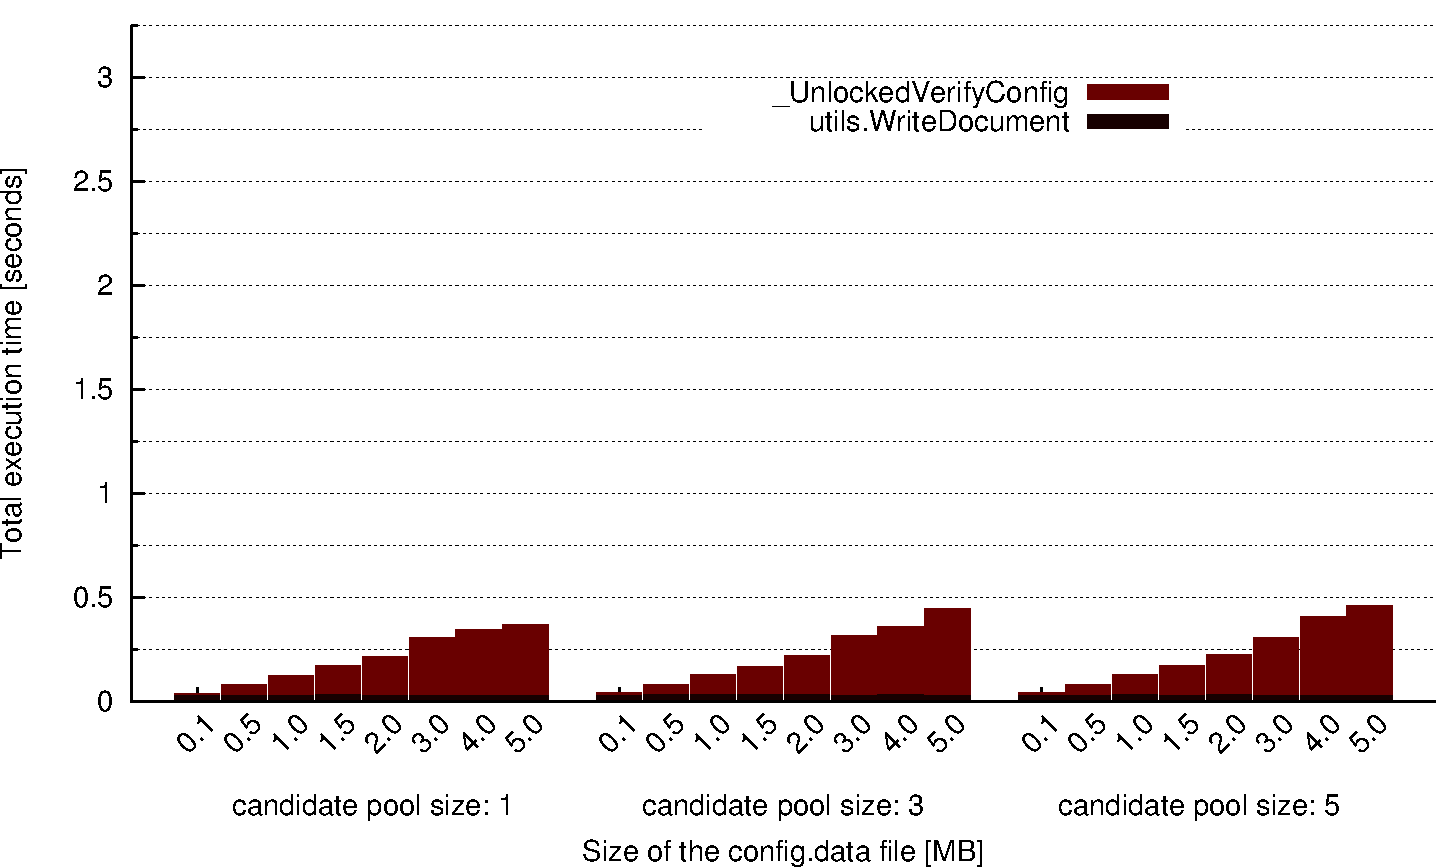
\includegraphics[width=1.0\maxwidth]{../figures/couchdb.pdf}
    \caption{Performance evaluation of the \_WriteConfig method of CouchDB}
    \label{fig:couchdb}
  \end{center}
\end{figure}

\begin{figure}[htbp]
  \begin{center}
    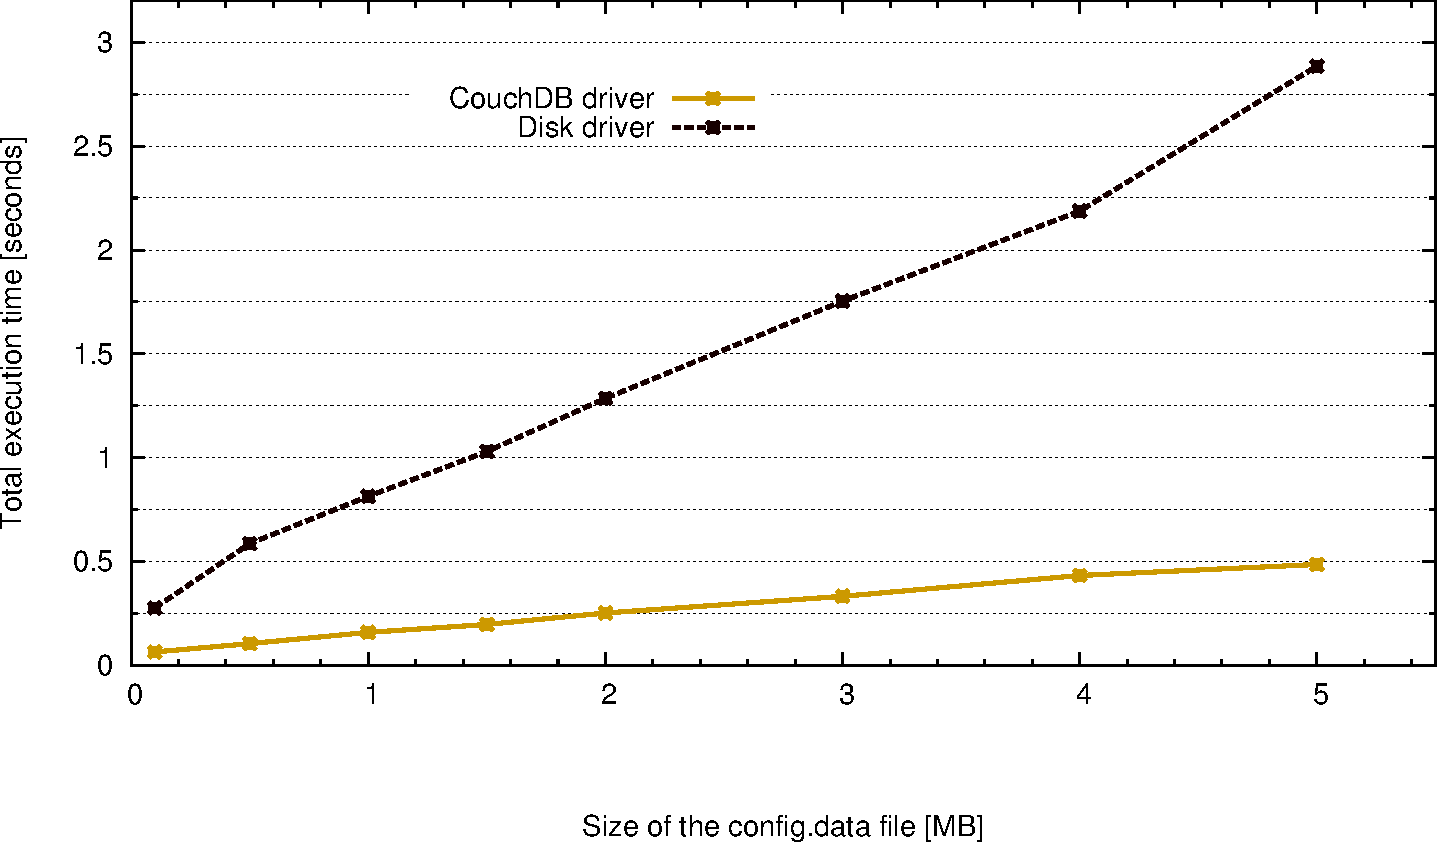
\includegraphics[width=1.0\maxwidth]{../figures/comp-cfg.pdf}
    \caption{Comparison of execution performance for instance modify ops}
    \label{fig:comp-cfg}
  \end{center}
\end{figure}

\subsection{Aggregate evaluation of the CouchDB driver}\label{subsec:total_eval}

Up to this point, we have tested our implementation in a variety of situations
that may occur in a Ganeti cluster. We also examined some of the main factors
that limit Ganeti from scaling and achieving better performance. In this last
benchmark category, we will attempt to measure the overall performance of
our drivers in a real-world scenario. In order to explain the results of this
section, we will also make use of the findings from the previous categories.

In a Ganeti cluster with \emph{5 vm-capable} nodes, and three master candidates,
we will concurrently submit jobs of \emph{OpInstanceCreate} opcodes, in batches
of \texttt{1}, \texttt{10}, \texttt{20}, \texttt{50}, and \texttt{100} jobs. We
will measure the average time of the phases that a job passes through, and then
the total execution duration from the first job that it is enqueued since the
last that is completed. Since the \texttt{Running} times of the jobs are
independent to the underlying storage layer that it is used, we will minimize
it by creating instances with \emph{1 GB} file disk, using the
\emph{--no-install}, \emph{--no-start} options that disable the OS installation
and the start-up of the instances respectively.

\bigskip
\newpage
\textbf{Performance Analysis}

Figure~\ref{fig:jobs_avg}, displays the average duration of the execution phases
of the \emph{InstanceCreate} jobs we submitted. For a short reminder about the
execution phases of a job, refer to Section~\ref{subsec:jobs}.

\begin{figure}[htbp]
  \begin{center}
    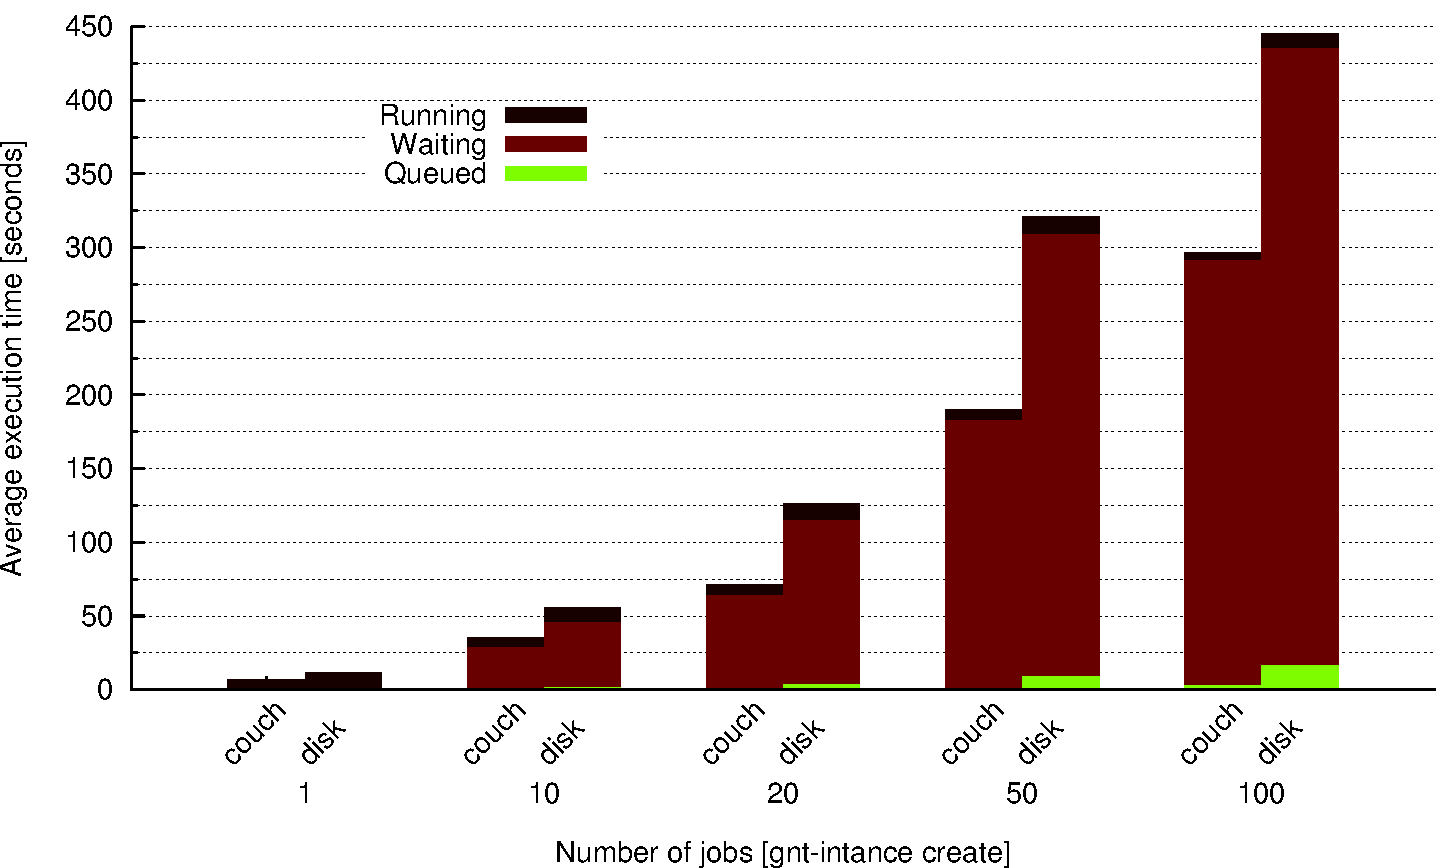
\includegraphics[width=1.0\maxwidth]{../figures/jobs_avg.pdf}
    \caption{Comparison of execution performance for the phases of a job}
    \label{fig:jobs_avg}
  \end{center}
\end{figure}

What we observe from Figure~\ref{fig:jobs_avg}, is a minimized \emph{Running}
time for reasons we already covered, while the most time is consumed in the
\emph{Waiting} phase. In this phase the jobs are waiting for locks, held by other
threads that are in execution. The \emph{Opportunistic locking} that it is used
since Ganeti version \emph{2.7}, improved the lock congestion in instance create
operations, but since we create a lot of instances in a small cluster, it is a
normal behavior. It is also observed that the average time of CouchDB in the
\emph{Queued}, and \emph{Waiting} phase is quite smaller comparing to the disk
implementation. We already covered the improved performance in the submission
rate of CouchDB. The new finding, is the increase in the average \emph{Waiting}
performance time. This behavior can be justified by the increased job submission
rate, as we presented in Figure~\ref{fig:comp}. The worker threads, are waiting
in the queue for new jobs to appear. As soon as a job is submitted in the queue,
and a worker thread is available, it grubs it for execution. An increased job
enqueue rate translates to workers that acquire their workload earlier. As a
result, we have an immediate impact in the \emph{Waiting} average time, due to
the fact that the workers are idle for less time than they previously were, and
the resources of the cluster are exploited more efficient than before. An
immediate consequence of the increase in the performance of the \emph{Queued}
and \emph{Waiting} time, is an increase in the total execution duration of the
jobs. This induction is justified by~Figure~\ref{fig:total_secs}.

\begin{figure}[htbp]
  \begin{center}
    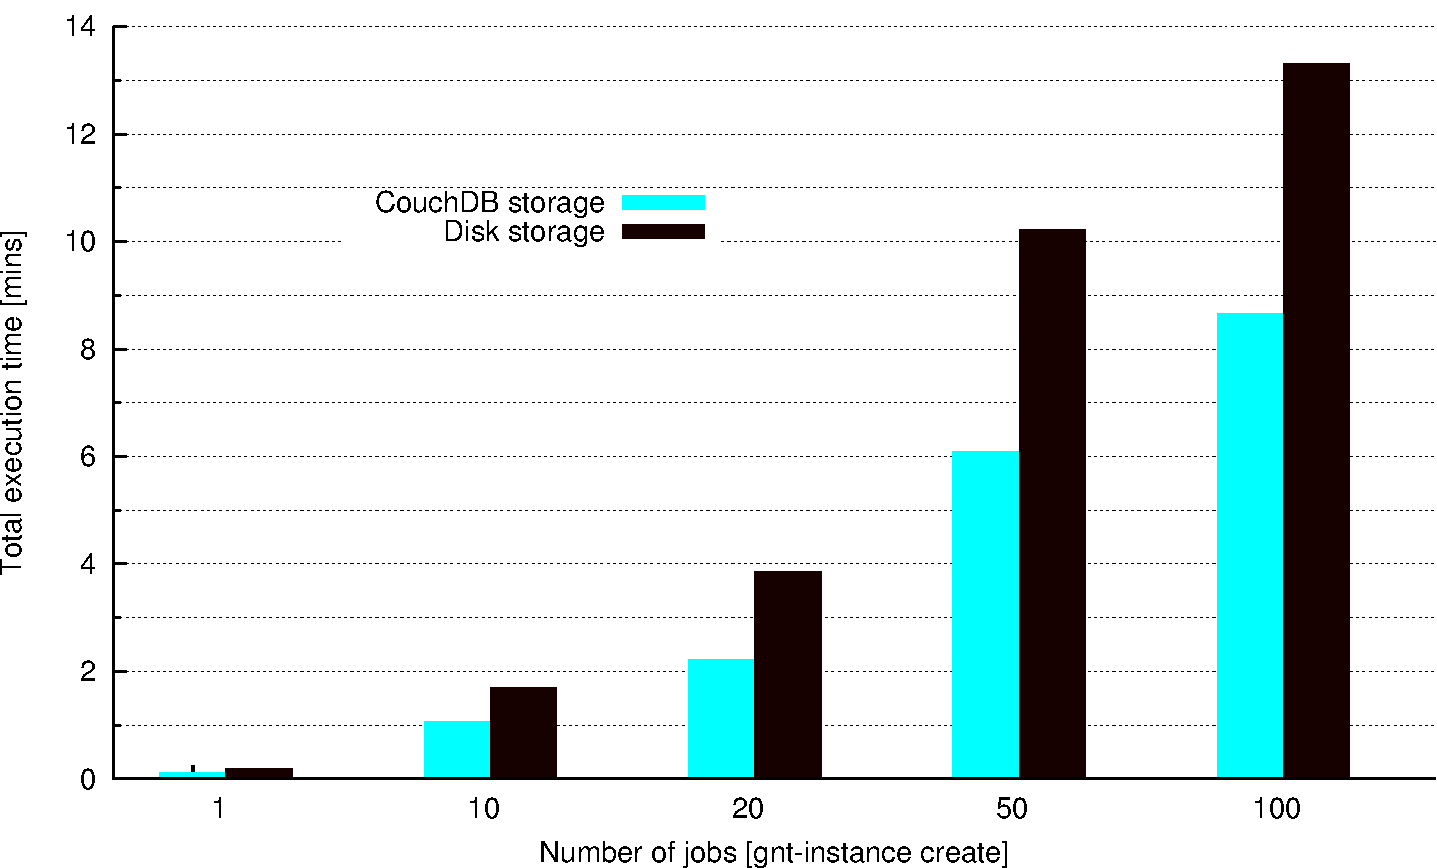
\includegraphics[width=1.0\maxwidth]{../figures/total_secs.pdf}
    \caption{Comparison of the throughput performance for instance create ops}
    \label{fig:total_secs}
  \end{center}
\end{figure}

What we conclude from Figure~\ref{fig:total_secs}, is that the CouchDB driver
performs better under a heavy loaded environment. The performance gap between
the two implementations widens as the number of jobs in the cluster increases.
CouchDB is designed to service highly concurrent use cases, and perform under a
heavy application load. The \emph{Multi-Version Concurrency Control} that
implements, makes CouchDB able to handle a high volume of concurrent readers and
writers without conflicts to each other. As a result, there will not appear any
performance gaps as the cluster workload is increased, and the requests will
continue to be serviced efficiently.
